\documentclass[unicode,a4paper,11pt]{ltjsarticle}

\usepackage{luatexja-fontspec}
\setmainfont{TeX Gyre Termes}
\setmainjfont[BoldFont = IPAGothic]{IPAMincho}
\setmathrm{Latin Modern Roman}
% \setmainjfont{Noto Sans JP}

% ---Display \subsubsection at the Index
% \setcounter{tocdepth}{3}

% ---Setting about the geometry of the document----
% \usepackage{a4wide}
% \pagestyle{empty}

% ---Physics and Math Packages---
\usepackage{amssymb,amsfonts,amsthm,mathtools}
\usepackage{physics,braket,bm}

% ---underline---
\usepackage[normalem]{ulem}

% ---cancel---
\usepackage{cancel}

% --- surround the texts or equations
% \usepackage{fancybox,ascmac}

% ---settings of theorem environment---
\theoremstyle{definition}
\newtheorem{dfn}{定義}
\newtheorem{prop}{命題}
\newtheorem{thm}{定理}
\newtheorem{exm}{例}
\newtheorem{exc}{演習}

% ---settings of proof environment---
\renewcommand{\proofname}{\textbf{証明}}
\renewcommand{\qedsymbol}{$\blacksquare$}

% ---Ignore the Warnings---
\usepackage{silence}
\WarningFilter{latexfont}{Some font shapes}
\WarningFilter{latexfont}{Font shape}
\WarningFilter{latexfont}{Size substitutions}
\ExplSyntaxOn
\msg_redirect_name:nnn{hooks}{generic-deprecated}{none}
\ExplSyntaxOff

% ---Insert the figure (If insert the `draft' at the option, the process becomes faster.)---
\usepackage{graphicx}
% \usepackage{subcaption}

% ----Add a link to a text---
\usepackage{url,hyperref}
\usepackage[dvipsnames,svgnames]{xcolor}
\hypersetup{colorlinks=true,citecolor=FireBrick,linkcolor=Navy,urlcolor=purple}
% ---refer `texdoc xcolor' at the command line---

% ---Tikz---
% \usepackage{tikz,pgf,pgfplots,circuitikz}
% \pgfplotsset{compat=1.15}
% \usetikzlibrary{intersections,arrows.meta,angles,calc,3d,decorations.pathmorphing}

% ---Add the section number to the equation, figure, and table number---
\makeatletter
   \renewcommand{\theequation}{$\thesection.\arabic{equation}$}
   \@addtoreset{equation}{section}
   
   \renewcommand{\thefigure}{\thesection.\arabic{figure}}
   \@addtoreset{figure}{section}
   
   \renewcommand{\thetable}{\thesection.\arabic{table}}
   \@addtoreset{table}{section}
\makeatother

% ---enumerate---
% \renewcommand{\labelenumi}{$\arabic{enumi}.$}
% \renewcommand{\labelenumii}{$(\arabic{enumii})$}

% ---Index---
% \usepackage{makeidx}
% \makeindex 

% ---Fonts---
% \renewcommand{\familydefault}{\sfdefault}

% ---Title---
\title{ペスキンゼミ\ 11章から13章}
\author{宮根 一樹}
\date{最終更新日:\today}

\begin{document}

\maketitle

\tableofcontents

\vspace*{10pt}

卒論発表前後のときとは打って変わってとっても元気なので、ゼミ資料とか作ってみました。勢いに任せているので、クオリティはあまり保証しません。それ以前に、ぺスキンのここらへんは評判良くないらしいですし、僕もそう思います。ですので、僕が犠牲になって(この地雷パートの)雰囲気だけは伝えられたらなと思います。

\vspace*{10pt}

\begin{itemize}
   \item
         春の学校の発表の準備や、研究の進捗があまり芳しくありません。全てはこのゼミ資料のせいです。これを身代わりに助かりたいところですが、まあ、そんなわけにはいかないでしょう。頑張ります。
   \item
         ファインマンダイアグラムを書くのがきつい。もう少し時間があったらちゃんとやったのですが。
   \item
         Youtubeを見てたら、深夜の首都高一周ドライブをしたくなりました。これを読んだ誰か、一緒に行きましょう。別に危ないことをしたいわけじゃないです。「山手線を徒歩/チャリ/電車で一周しました!」って人たちと同じモチベーションです。
\end{itemize}

\clearpage

\section{くりこみと対称性}

対称性というのがQFT(というか物理全般)で大事なのは周知のこととは思いますが、では、くりこみをした後の物理では、もとの対称性はどうなっているのでしょうか?素朴に考えれば、くりこみでやってることは、ラグランジアンのパラメターをいじることだけですので、ラグランジアン自体の対称性は変わらないような気がするのですが、量子補正は物理量を変えてしまうため、得られる物理量は対称性を反映していない可能性もありそうです。この章では、まずは古典レベルで一部の対称性を破っておいて、くりこんだ理論がどうなるかどうかを見ていきます。

得られる結果としては
\begin{itemize}
   \item
         古典論のレベルでは、対称性を破ると質量が0の粒子が生成される(ゴールドストーンの定理, \S11.1)
   \item
         任意のオーダーでくりこみをした後でも、ゴールドストーンの定理は成立する(\S11.2,\S11.6)
\end{itemize}
ということです\footnote{
   個人的に導入で結論まで言ってしまう構成が好きなので、この資料ではこのスタイルで行こうと思います。
}。特に、2つめの項目を議論するときに、量子補正も取り込んだ有効的な作用を書いておくと見通しがいいので、ここではそれらの道具の整備についても議論していきます。


\subsection{対称性の破れとゴールドストーンの定理}

ここでは、古典レベルで対称性を一部だけ破る例として、$O(N)$対称性のある線形シグマ模型を見ていきます。ラグランジアンは、$\phi^{i}\ (i=1,\cdots,N)$をスカラー場として
\begin{equation}
   \mathcal{L}
   =
   \frac{1}{2}(\partial_{\mu}\phi^{i})^2
   +
   \frac{1}{2}\mu^2(\phi^{i})^2
   -
   \frac{\lambda}{4}[(\phi^{i})^2]^2
   \label{eqn:lagrangian_N_linearsigma}
\end{equation}
です。ただし、$[(\phi^{i})^2]^2\equiv [(\phi^{1})^2+\cdots+(\phi^{N})^2]^2$です。この理論は$\phi^{i}$のノルムでかけているので、$N\times N$の直交行列$R\in O(N)$で回す変換に対して不変です。実際、${\phi^{i}}^{\prime}\equiv R^{ij}\phi^{j}$とすれば
\begin{equation}
   ({\phi^{i}}^{\prime})^2
   =
   \phi^{k}R^{ki}\cdot R^{ij}\phi^{j}
   =
   (\phi^{i})^2
\end{equation}
です。この理論のポテンシャルは
\begin{equation}
   V(\phi)
   =
   -\frac{1}{2}\mu^2 (\phi^{i})^2+\frac{\lambda}{4}[(\phi^{i})^2]^2
\end{equation}
ですが、最小点は
\begin{equation}
   (\phi^{i})^2
   \frac{\mu^2}{\lambda}
\end{equation}
であり、そのような点は複数あります。そのような点の中から、ここでは真空期待値を
\begin{equation}
   \phi_{0}^{i}
   =
   (0,0,\cdots,v)
   ,\
   v\equiv\frac{\mu}{\sqrt{\lambda}}
\end{equation}
ととりましょう。この最小点で場$\phi^{i}$を展開すると
\begin{equation}
   \phi^{i}
   =
   (\pi^{1},\pi^{2},\cdots,\pi^{N-1},v+\sigma(x))
\end{equation}
と書けるので、ラグランジアン\eqref{eqn:lagrangian_N_linearsigma}を新しい場$\pi^{k},\sigma$で書き換えると
\begin{align}
   \mathcal{L}
    & =
   \frac{1}{2}(\partial_{\mu}\pi^{k})^2
   +
   \frac{1}{2}(\partial_{\mu}\sigma)^2
   -
   \frac{1}{2}(2\mu^2)\sigma^2
   \nonumber
   \\
    & \qquad
   -\sqrt{\lambda}\mu\sigma^3
   -\sqrt{\lambda}\mu(\pi^{k})^2\sigma
   -\frac{\lambda}{4}\sigma^4
   -\frac{\lambda}{2}(\pi^{k})^2\sigma^2
   -\frac{\lambda}{4}[(\pi^{k})^2]^2
   \label{eqn:lagrangian_N_linearsigma_2}
\end{align}
となります。ただし、定数は無視しています。

この理論についての量子論は次節から取り扱うとして、古典論のレベルから分かることは、$(N-1)$個の無質量な場$\pi^{k}$が現れていることです。今、$\pi^{k}$についての対称性が$O(N-1)$として残っているわけですが、このように対称性が敗れると質量がある理論から無質量な粒子が出ることが分かっており、これを\textbf{ゴールドストーンの定理}といいます。また、この自発的対称性の破れによって生じた無質量な粒子を\textbf{ゴールドストーンボソン}といったりします。

ゴールドストーンの定理は教科書に証明があるので、ここでは省略します。読書の手助けのために、その証明のスケッチを述べておくと
\begin{enumerate}
   \item
         ポテンシャルをVEVの周りで展開して、その2次の係数が質量行列なのだからそこをみる。
   \item
         もし、そのVEVでは元の対称性が保っていないなら、その分だけ質量行列のランクが削れて固有値に0が含まれることになる。
\end{enumerate}
といった感じです。


\subsection{くりこみと対称性の具体例}

線形シグマ模型\eqref{eqn:lagrangian_N_linearsigma_2}を量子化しましょう。すると、場$\pi^{k}(x),\sigma(x)$のファインマンダイアグラムはすぐに求まります、が、どうせすぐにくりこみを議論するためにラグランジアンを書き換えるのでここでは書きません。ラグランジアンの書き換えは、元々のラグランジアン\eqref{eqn:lagrangian_N_linearsigma}には3つの発散するパラメターがあったことから、$\phi^{i}\rightarrow Z\phi^{i}$とリスケーリングしたあとに
\begin{equation}
   \delta_{Z}
   \equiv
   Z-1
   ,\
   \delta_{m}
   \equiv
   m_{0}^2Z-m^2
   ,\
   \delta_{\lambda}
   \equiv
   \lambda_{0}Z^2
   -
   \lambda
\end{equation}
と裸の定数を書き換えてやれば、
\begin{equation}
   \mathcal{L}
   \equiv
   \mathcal{L}_{\mathrm{phys.}}+\mathcal{L}_{\mathrm{c.t.}}
\end{equation}
と物理的な項$\mathcal{L}_{\mathrm{phys.}}$と相殺項$\mathcal{L}_{\mathrm{c.t.}}$に分離できます。$\mathcal{L}_{\mathrm{phys.}}$のほうは\eqref{eqn:lagrangian_N_linearsigma_2}と同じで、相殺項のほうは
\begin{align}
   \mathcal{L}_{\mathrm{c.t.}}
    & =
   \frac{\delta_{Z}}{2}(\partial_{\mu}\pi^{k})^2
   -
   \frac{1}{2}(\delta_{\mu}+\delta_{\lambda}v^2)(\pi^{k})^2
   +
   \frac{\delta_{Z}}{2}(\partial_{\mu}\sigma^2)^2
   -
   \frac{1}{2}(\delta_{\mu}+3\delta_{\lambda}v^2)\sigma^2
   \nonumber
   \\
    & \qquad
   -
   (\delta_{\mu}v+\delta_{\lambda}v^3)\sigma
   -
   \delta_{\lambda}v\sigma(\pi^{k})^2
   -
   \delta_{\lambda}v\sigma^3
   -
   \frac{\delta_{\lambda}}{4}[(\pi^{k})^2]^2
   -
   \frac{\delta_{\lambda}}{2}\sigma^{2}(\pi^{k})^2
   -
   \frac{\delta_{\lambda}}{4}\sigma^4
   \label{eqn:lagrangian_N_linearsigma_counter}
\end{align}
と書けます。したがって、\eqref{eqn:lagrangian_N_linearsigma_2}と\eqref{eqn:lagrangian_N_linearsigma_counter}からファインマンダイアグラムは教科書の図11.3のようになります。

この理論には、相殺項が3つ$\delta_{Z},\delta_{\mu},\delta_{\lambda}$しかありません。したがって、くりこみ条件を3つ用意して発散を相殺しようと思うわけですが、理論が複数の頂点をもつことから、3つのパラメターチューニングだけで発散が消せるかどうかは自明ではないように思います。もし、3つのくりこみ条件が足りないなら、新たに相殺項を導入することによって発散を消そうと思うわけですが、それはラグランジアンの対称性をさらに破る可能性が考えられます。

しかしながら、少なくともone-loopのレベルでのくりこみは、上のゴールドストーンの定理を破らないことが分かっているので、ここでは愚直に計算してその事実を確認してみましょう。まずはくりこみ条件ですが、ここでは以下のようにします:
\begin{align}
   \vcenter{\hbox{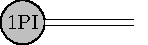
\includegraphics{fig/11_17_1.pdf}}}
    & =
   0
   ,
   \label{eqn:renorm_cond_1}
   \\
   \dv{}{p^2}
   \left(
   \vcenter{\hbox{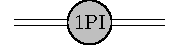
\includegraphics{fig/11_17_2.pdf}}}
   \right)
    & =
   0
   \qquad
   (p^2=m^2)
   ,
   \label{eqn:renorm_cond_2}
   \\
   \vcenter{\hbox{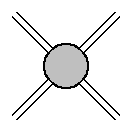
\includegraphics{fig/11_17_3.pdf}}}
    & =
   -6i\lambda
   .
   \label{eqn:renorm_cond_3}
\end{align}
1つめの条件はVEVのシフトを無視して簡単にするための条件、残り2つは$m,\lambda$を決めるための条件に対応しているそうです。まずは3つめの条件\eqref{eqn:renorm_cond_3}を見ていきます。この条件は発散を相殺する頂点も併せて条件を考えてやると、教科書の式(11.18)が$-6i\lambda$になればよいです\footnote{
   教科書の$\mathrm{Im}$はタイポ?
}。ただし、crossesのところは、ダイアグラムの形が変わるところで、教科書の326ページの式の最初の式の第1項みたいな感じです。計算は省略しますが、これらの条件の漸近的なふるまいから$\delta_{\lambda}$が決まって
\begin{equation}
   \delta_{\lambda}
   \sim
   \lambda^{\lambda}(N+8)\frac{\Gamma(2-d/2)}{(4\pi)^2}
\end{equation}
です。

同様にして、残りの$\delta_{\mu},\delta_{Z}$を決めましょう。条件\eqref{eqn:renorm_cond_1}は
\begin{equation}
   \vcenter{\hbox{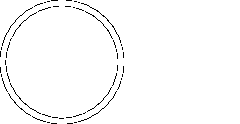
\includegraphics{fig/11_30_1.pdf}}}
   +
   \vcenter{\hbox{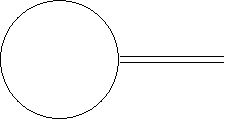
\includegraphics{fig/11_30_2.pdf}}}
   +
   \vcenter{\hbox{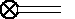
\includegraphics{fig/11_30_3.pdf}}}
   =
   0
\end{equation}
に対応していて、これを計算すると
\begin{equation}
   \delta_{\mu}
   +
   v^2\delta_{\lambda}
   =
   -\lambda\frac{\Gamma(1-d/2)}{(4\pi)^{d/2}}
   \left(
   \frac{3}{(2\mu^2)^{1-d/2}}
   +
   \frac{N-1}{(\zeta^2)^{1-d/2}}
   \right)
\end{equation}
から$\delta_{\mu}$が決まります(既に$\delta_{\lambda}$は知っているので)。残りは条件\eqref{eqn:renorm_cond_2}ですが、これを書き下すと
\begin{equation}
   \dv{}{p^2}
   \left(
   \vcenter{\hbox{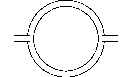
\includegraphics{fig/11_34_1.pdf}}}
   +
   \vcenter{\hbox{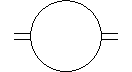
\includegraphics{fig/11_34_2.pdf}}}
   +
   \vcenter{\hbox{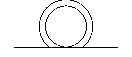
\includegraphics{fig/11_34_3.pdf}}}
   +
   \vcenter{\hbox{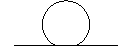
\includegraphics{fig/11_34_4.pdf}}}
   +
   \vcenter{\hbox{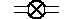
\includegraphics{fig/11_34_5.pdf}}}
   \right)
   =
   0
\end{equation}
となりますが、実はこれを計算すると$\delta_{Z}=0$でよいことが分かります。

以上の議論で、くりこみ定数がもとまったわけですが、これらの定数から他の発散のあるダイアグラムが消えるかどうかは調べる必要があります。教科書はいくつかやっているので、ここでは後の議論に関わってくる$\pi$の2点振幅を見ていきましょう。そのためには$\pi$と$\pi$の相殺項を見ればよいのですが、それは教科書の式(11.37)のようになります。このダイアグラムはこれまでにもとめた$\delta_{\lambda},\delta_{\mu},\delta_{Z}$によってちょうど有限になることが計算から分かるのですが、そもそも$p=0$でその値が0になることが分かります。このダイアグラムの極が質量の場所を示すわけですが、そもそも0なら極なしで質量はありませんので$\pi$は質量なし、と結論付けられるわけです。


\subsection{有効作用}

前節では、くりこみ条件をうまくとることによってVEVのシフトが起こらないようにしていましたが、一般にはそういったことが起こりえます。VEVは古典的にはポテンシャルの最小点であるわけですが、量子補正が入るとVEVが最小点からずれる可能性があります。量子補正を取り込んだVEVも\textbf{量子効果込みの}新しいポテンシャルの最小点になっているはずですので、そのようなポテンシャルをもとめる手続きを考えよう、というのが今後の目標になります。このときに、熱力学のギブスポテンシャルが参考になります。ギブスエネルギーは、ヘルムホルツの自由エネルギーをルジャンドル変換して得られるわけですが、この最小点が熱力学的に安定な状態となります\footnote{
   もちろん、ヘルムホルツの自由エネルギーを最小化するところも安定点なのですが、それは見ている変数が違います。今回は、分配関数から始める都合上、変数はヘルムホルツよりもギブスのものがいいっていう感じなんじゃないでしょうか。完全に私の憶測ですが。
}。

お話はこれぐらいにしておいて、分配関数が
\begin{equation}
   Z[J]
   =
   \int\mathcal{D}\phi\
   \exp
   \left[
      \mathcal{L}+J\phi
      \right]
   \equiv
   e^{-i E[J]}
\end{equation}
と書けると思いましょう。ここで、$E[J]$はヘルムホルツの自由エネルギーに対応するものです。したがって、これを$J$で微分したものが場$\phi$の真空期待値になっているはずなので、これを
\begin{equation}
   \phi_{\mathrm{c}}
   \equiv
   -
   \frac{\delta}{\delta J(x)}E[J]
\end{equation}
と定義しておきましょう\footnote{
   これはスピン系に外場をかけたときに、スピンが平均してどの向きに傾くのかに対応しています。
}。と、すると、これをむしろ1つの変数だとみなすポテンシャルがルジャンドル変換によって得られるので、それを
\begin{equation}
   \Gamma[\phi_{\mathrm{c}}]
   \equiv
   -
   E[J]
   -
   \int\dd^4 y\
   J(y)\phi_{\mathrm{c}}(y)
\end{equation}
と書くことにします。この$\Gamma[\phi_{\mathrm{c}}]$を\textbf{有効作用}と呼び、これらが時空の体積$V\cdot T$に比例しているとしたとき、その係数
\begin{equation}
   V_{\mathrm{rff}}[\phi_{\mathrm{c}}]
   \equiv
   -\frac{1}{VT}\Gamma[\phi_{\mathrm{c}}]
\end{equation}
を\textbf{有効ポテンシャル}とよぶことにします。これらは、
\begin{align}
   \frac{\delta}{\delta \phi_{\mathrm{c}}(x)}E[J]
    & =
   -
   \frac{\delta}{\delta \phi_{\mathrm{c}}(x)}
   -
   \frac{\delta}{\delta \phi_{\mathrm{c}}(x)}
   \int\dd^4 y\
   J(y)\phi_{\mathrm{c}}(y)
   \nonumber
   \\
    & =
   -J(x)
\end{align}
となることから、$J=0$のときはVEVが古典レベルのVEVと一致します。

実は、この手続きはもともとのポテンシャルを強引に凸関数にして準安定な真空をつぶしていることに対応するのですが、これの説明については省略します。とにかく、この有効ポテンシャル$V_{\mathrm{rff}}[\phi_{\mathrm{c}}]$が計算できれば、後は視覚的にVEVの位置が分かるので非常に有用です。


\subsection{有効作用の計算}

実際に今の文脈で計算する方法を見ていきます。まず、ラグランジアンは
\begin{equation}
   \mathcal{L}
   =
   \mathcal{L}_{1}
   +
   \delta\mathcal{L}
\end{equation}
と物理的な項$\mathcal{L}_{1}$と相殺項$\delta\mathcal{L}$に分けておきます。

摂動の0次では、その解は古典解$\phi_{\mathrm{c}}$のはずなので、
\begin{equation}
   \left.
   \frac{\delta\mathcal{L}}{\delta\phi}
   \right|_{\phi=\phi_{\mathrm{c}}}
   +
   J
   =
   0
\end{equation}
が成立しています(紛らわしくてぶん殴りたくなりますが、第1項は変分ですのでそれ自体が運動方程式です)。ここで、$J_{1}$をこのうち相殺項を除いた方程式
\begin{equation}
   \left.
   \frac{\delta\mathcal{L}_1}{\delta\phi}
   \right|_{\phi=\phi_{\mathrm{c}}}
   +
   J_{1}
   =
   0
\end{equation}
で定義しておきます。後は$\delta J\equiv J-J_{1}$としておけば、相殺項は分離できて
\begin{equation}
   e^{-i E[J]}
   =
   \int\mathcal{D}\phi\
   \exp
   \left[
   i\int\dd^4 x\
   (\mathcal{L}_{1}+J_{1}\phi)
   \right]
   \exp
   \left[
      i\int\dd^4 x\
      (\delta\mathcal{L}+\delta J\phi)
      \right]
\end{equation}
となります。後ろのほうはいったん忘れて、1つめの因子に注目しましょう。今回やりたいのは、古典場$\phi=\phi_{\mathrm{c}}$が従うポテンシャルを有効的に書き下してやることですので、その周りで展開して
\begin{align}
   \mathcal{L}_{1}+J_{1}\phi
    & =
   \left(
   \mathcal{L}_{1}[\phi_{\mathrm{c}}]+J_{1}\phi_{\mathrm{c}}
   \right)
   +
   \left(
   \frac{\delta\mathcal{L}_{1}}{\delta\phi}[\phi_{\mathrm{c}}]
   +
   J
   \right)\eta
   \nonumber
   \\
    & \qquad
   +
   \frac{1}{2}\int\dd^4 y\
   \frac{\delta^2 \mathcal{L}_1}{\delta\phi(x)\delta\phi(y)}[\phi_{\mathrm{c}}]\eta(x)\eta(y)
   +
   \cdots
\end{align}
としておきます。ただし、$\eta\equiv\phi-\phi_{\mathrm{c}}$。$\eta$の1次は古典解の条件から消えて、2次以降が量子補正となります。経路積分の変数を$\phi$から$\eta$に変えて、最初の補正を加えた部分を見ると
\begin{equation}
   \int\mathcal{D}\eta\
   \exp
   \left[
   i
   \left(
   \int\dd^4 x (\mathcal{L}_{1}[\phi_{\mathrm{c}}]+J\phi_{\mathrm{c}})
   \right)
   \right]
   \cdot
   \exp
   \left[
      \frac{1}{2}
      \int\dd^4 x\dd^4 y\
      \eta\frac{\delta^2\mathcal{L}_{1}}{\delta\phi\delta\phi}\eta
      \right]
\end{equation}
となっており、量子補正のほうはガウシアンの積分なのでこれは行列式がでてきて
\begin{equation}
   \int\mathcal{D}\eta\
   \exp
   \left[
      \frac{1}{2}
      \int\dd^4 x\dd^4 y\
      \eta\frac{\delta^2\mathcal{L}_{1}}{\delta\phi\delta\phi}\eta
      \right]
   =
   \left(
   \mathrm{det\ }
   \left[
      -\frac{\delta^2\mathcal{L}_{1}}{\delta\phi\delta\phi}
      \right]
   \right)^{-1/2}
\end{equation}
です。この部分が量子補正として有効ポテンシャルに関わってきます。

線形シグマ模型を例に計算してみましょう。ラグランジアン
\begin{equation}
   \mathcal{L}_{1}
   =
   \frac{1}{2}(\partial_{\mu}\phi^{i})^2
   +
   \frac{1}{2}\mu^2 (\phi^{i})^2
   -
   \frac{\lambda}{4}[(\phi^{i})^2]^2
\end{equation}
を$\phi^{I}=\phi_{\mathrm{c}}^{I}$のまわりで展開すると
\begin{align}
   \mathcal{L}_{1}
    & =
   \frac{1}{2}(\partial_{\mu}\eta^{i})^2
   +
   \frac{1}{2}\mu^2 (\phi_{\mathrm{c}}^{i}+\eta^{i}(x))^2
   -
   \frac{\lambda}{4}[(\phi_{\mathrm{c}}^{i}+\eta^{i}(x))^2]^2
   \nonumber
   \\
    & =
   \frac{1}{2}(\partial_{\mu}\eta^{i})^2
   +
   \frac{1}{2}\mu^2(\phi_{\mathrm{c}^{i}})^2
   -
   \frac{\lambda}{4}[(\phi_{\mathrm{c}}^{i})^2]^2
   +
   (\mu^2-\lambda(\phi_{\mathrm{c}}^{i})^2)\phi_{\mathrm{c}}^{i}\eta^{i}
   \nonumber
   \\
    & \qquad
   +
   \frac{1}{2}\mu^2(\eta^{i})^2
   -
   \frac{\lambda}{2}[(\phi_{\mathrm{c}}^{i})^2(\eta^{i})^2+2(\phi_{\mathrm{c}}^{i}\eta^{i})^2]
   +
   \cdots
\end{align}
となります。この場合、$\eta^{i}$について2次なのは
\begin{equation}
   \frac{\delta^{2}}{\delta\eta^{i}\delta\eta^{j}}\mathcal{L}_{1}
   =
   -
   \delta^{ij}\partial^{2}
   +
   \mu^2\delta^{ij}
   -
   \lambda[(\phi_{\mathrm{c}}^{k})^2\delta^{ij}+2\phi_{\mathrm{c}}^{i}\phi_{\mathrm{c}}^{j}]
\end{equation}
です。ただし、変分をとっていることから第1項は微の形で残しておきます\footnote{
   固有値が作る行列です。
}。あとは、これの$\mathrm{det}$をとりたいのですが、VEVを決めてしまってもう少し計算を楽にしましょう。
































\end{document}
